\section{Design Patterns}
\subsection{Model View ViewModel (MVVM)}
\begin{figure}[H]
	\centering
	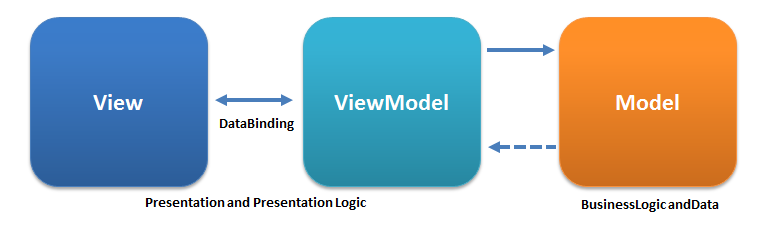
\includegraphics[scale=0.6]{Figures/WebImages/MVVMPattern}\\
	% place the figure in the Figures folder (located with the main file)
	% you need to fix the scale a few times to get it right, but latex does not compress so one can always zoom in to see details.
	\caption{The MVVM Pattern - http://en.wikipedia.org/wiki/Model\_View\_ViewModel}
	\label{fig:MVVMPattern}
	% label it something meanfull
\end{figure}
The \texttt{DriveIT Windows Client} uses the "Model View ViewModel" architectural pattern which tries to ensure a clear separation between the model and the view. 
\subsection{Observer pattern}

\subsection{Adapter patterns}
The adapter patterns allows the coder to encapsulate an object its methods and properties. The \texttt{DriveIT Windows Client} uses the MVVM design pattern originated from Microsoft, and it requires every view to have a corresponding Viewmodel, and furthermore The \texttt{DriveIT Web API} uses Data Transfer Objects(DTO) to send and receive data. Since DTO's are only meant to transfer data, no functions should exist in the class, therefore all Single Entitiy ViewModels in the \texttt{DriveIT.WindowsClient.ViewModels} name-space functions as Adapters for their corresponding DTO. E.g The CarViewModel class is an adapter for the CarDto class.\\ 

This implementation provides the WindowsClient with an easy way to manipulate data, while still remaining the data-structure such that it can be Created, Read, Updated and Deleted over the \texttt{DriveIT Web API} without converting.